\chapter{Introducción}
\label{chap:introduccion} 
La forma de impartir conocimientos ha ido cambiando y evolucionando a lo largo de los años. Actualmente es difícil no encontrar un aula donde las tecnologías web están muy presentes y más en el ambiente universitario. Para poder implementar una plataforma web competitiva en el mercado y además atrayente al usuario es imprescindible no sólo proporcionar la funcionalidad apropiada cumpliendo siempre con los requisitos de usabilidad correspondientes, sino que también es necesario conocer como los usuarios utilizan la plataforma. Para ello, es imprescindible recoger la interactividad que el usuario tiene con la plataforma web, guardar esos datos y después visualizarlos.\\

En este capítulo se va a hablar de los elementos clave en los que se basa este trabajo que son las tecnologías web, y la robótica educativa. También se introducirá en qué consiste un monitoreo y análisis de una página web.



%%%%%%%%%%%%%%%%%%%%%%%%%%%%%%%%%%%%%%%%%%%%%%%%%%%%%%%%%%%%%%%%%%%%%%%%%%%%%%%%%%%%%%%%%%%%%%%%%%%%%%%%%%%%%%%%
\section{Tecnologías web}\label{motivacion}
Las tecnologías de internet se remontan a 1970, cuando el departamento el departamento de defensa de Estados Unidos creó una red descentralizada la cual pudiera aguantar ataques nucleares. En 1990, Tim Berners-Lee trabajador del CERN\footnote{Organización Europea para la Investigación Nuclear} originó un protocolo de comunicación basado en hipertextos (HTTP) donde científicos compartían documentos, gracias a eso Berners-Lee junto a su equipo desarrolló el lenguaje de marcado HTML\footnote{HyperText Markup Language} y el sistema de direcciones de web URL\footnote{Uniform Resource Locator}, ese mismo año creó la primera página web (Figura 1.1) dando inicio a la WWW\footnote{World Wide Web}. Al cabo de los años se fueron desarrollando los diferentes navegadores hasta los que se conocen hoy en día. \\

\begin{figure}[H]
    \centering
    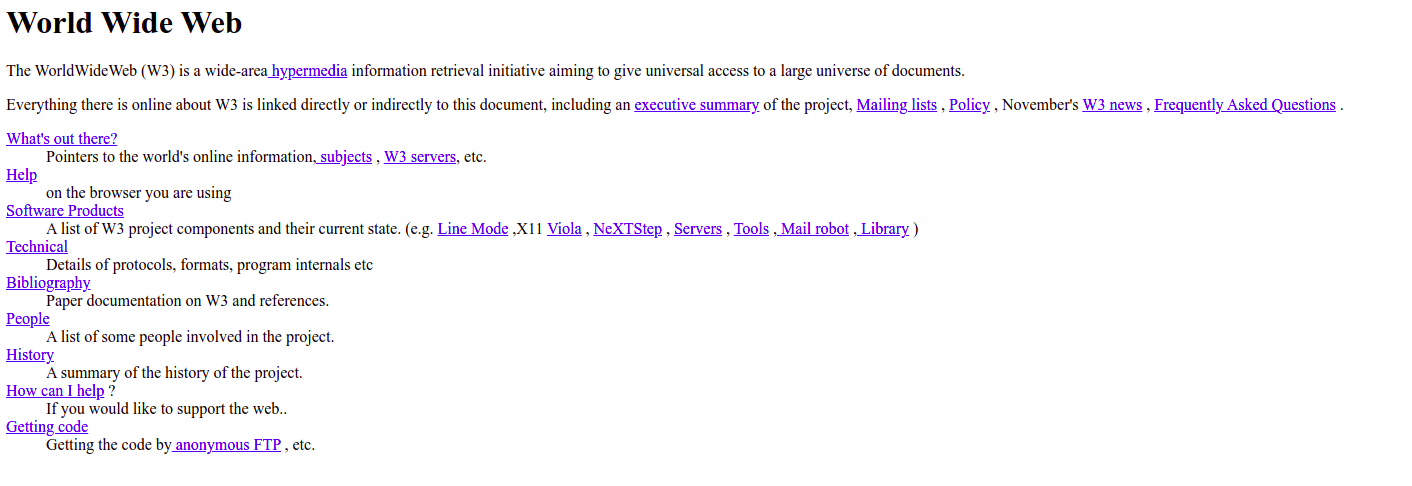
\includegraphics[width=16cm, keepaspectratio]{img/first_web_page.png}
    \caption{Primera página web}
    \label{fig:web}
\end{figure}

En la actualidad las principales ventajas de las tecnologías web son que se pueden utilizar en cualquier dispositivo, el usuario no necesita instalar nada más allá de un navegador web y su usabilidad es sencilla, si bien es necesaria una conexión a Internet para poder acceder a ellas \cite{juan}.\\

Las páginas Web modernas utilizan el modelo Cliente-Servidor, en el que el cliente hace peticiones al servidor esperando una respuesta de éste. Un mismo cliente puede estar conectado con varios servidores y a la vez interactúa con el usuario final normalmente a través de una interfaz gráfica. La parte del servidor se encarga de recibir las peticiones, analizarlas y procesarlas para enviar una respuesta. En las siguientes subsecciones, describimos algunas de las tecnologías más populares utilizadas en el desarrollo de páginas Web.

\begin{figure}[H]
    \centering
    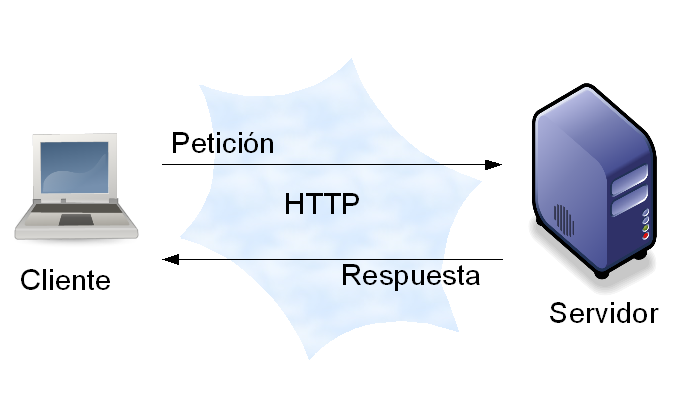
\includegraphics[width=10cm, keepaspectratio]{img/arquitectura.png}
    \caption{Arquitectura Cliente-Servidor}
    \label{fig:arquitectura}
\end{figure}

\subsection{Tecnologías web del lado del cliente}
Las tecnologías del lado del cliente suelen recibir el nombre de \textit{frontend}, son las que interactúan con el usuario, las más importantes son:

\begin{itemize}
  \item \textbf{HTML}:  Lenguaje de marcado que se encarga de dar la estructura a la página web. HTML utiliza etiquetas para mostrar los diferentes contenidos. La última versión es HTML5 donde se introducen las etiquetas de audio y vídeo.
  \item \textbf{CSS} \footnote{Cascading Style Sheets}: Lenguaje de estilo que se encarga del diseño gráfico, de la apariencia de las páginas web. La última versión es CSS3.
  \item \textbf{JavaScript}: Lenguaje de programación interpretado que permite la ejecución de código orientado a eventos (por ejemplo, pulsar un botón). Puede actuar sobre el navegador a través de objetos integrados, es decir puede manipular el HTML.
\end{itemize}

\subsection{Tecnologías web del lado del servidor}
Las tecnologías web del lado del servidor, también llamadas \textit{backend}, son las encargadas de procesar las peticiones del cliente y enviar una respuesta en forma de páginas HTML. Normalmente se utilizan \textit{frameworks }que son herramientas que te permiten desarrollar una aplicación web de forma ágil y sencilla a partir de librerías o funciones ya creadas. Algunos de estos \textit{frameworks} son:

\begin{itemize}
\item \textbf{Django}: Basado en Python. Django hace uso de plantillas permitiendo hacer páginas web más rápidas y sencillas. Gracias a su ORM \footnote{Object Relational Mapping} no es necesario saberse el manejo de base de datos ya que este traduce directamente el código de Python al lenguaje estándar de las peticiones a bases de datos, SQL.
\item \textbf{Node.js}: Permite ejecutar código JavaScript fuera del navegador y está construido con el motor de JavaScript V8 de Chrome. Node.js utiliza un modelo de entrada y salida no bloqueante, no espera a que los procesos finalicen.
\item \textbf{Symfony}: Utiliza de lenguaje de programación PHP\footnote{Hypertext Preprocessor}. Está basado en el patrón Modelo Vista Controlador (MVC). Symfony es muy flexible permitiéndote instalar únicamente lo que se necesite en vez del \textit{framework} completo.
  \item \textbf{Spring Boot}: Desarrollado para aplicaciones programadas en Java, surgió debido a que el Spring Framework era difícil de configurar. 
\item \textbf{Lavarel}: \textit{Framework} de PHP. En comparación con otros \textit{frameworks } de PHP su curva de aprendizaje es más baja. Es flexible y adaptable, no solamente debido al MVC, sino que también propone utilizar \textit{routes with clousures}, a causa de lo cual reduce código \cite{lavarel}.
\end{itemize}

%%%%%%%%%%%%%%%%%%%%%%%%%
\section{Plataforma web de programación}
En la actualidad, gracias a Internet se tiene al alcance plataformas web donde se enseña a programar de una forma interactiva. Una de las ventajas de aprender programación en una plataforma web es que puedes hacer desde la comodidad de tu casa y una gran parte son gratuitas. Pueden ser utilizadas por usuarios de todos los niveles. A continuación, se nombra algunos ejemplos de estas plataformas:\\
\newpage
\begin{itemize}
\item \textbf{Scratch}\footnote{https://scratch.mit.edu/}: Es un entorno de programación desarrollado por el MIT\footnote{Massachusetts Institute of Technology}. Se puede descargar en local o se puede utilizar la plataforma de forma \textit{online}. Utiliza un lenguaje de programación visual llamado igual que la plataforma, Scratch, el cual está basado en bloques permitiendo crear programas arrastrando y soltando para agrupar dichos bloques como un puzle. Cada bloque puede significar un evento, movimiento, un operador o una variable, entre otras. Con esta plataforma, por ejemplo, se pueden crear juegos, historias interactivas, música de manera sencilla y dinámica para el usuario. Las edades que tienen los usuarios que utilizan la plataforma esta entre los 8 y 16 años, aunque hay adultos que también la utilizan \cite{scratch}.
\end{itemize}

\begin{figure}[H]
    \centering
    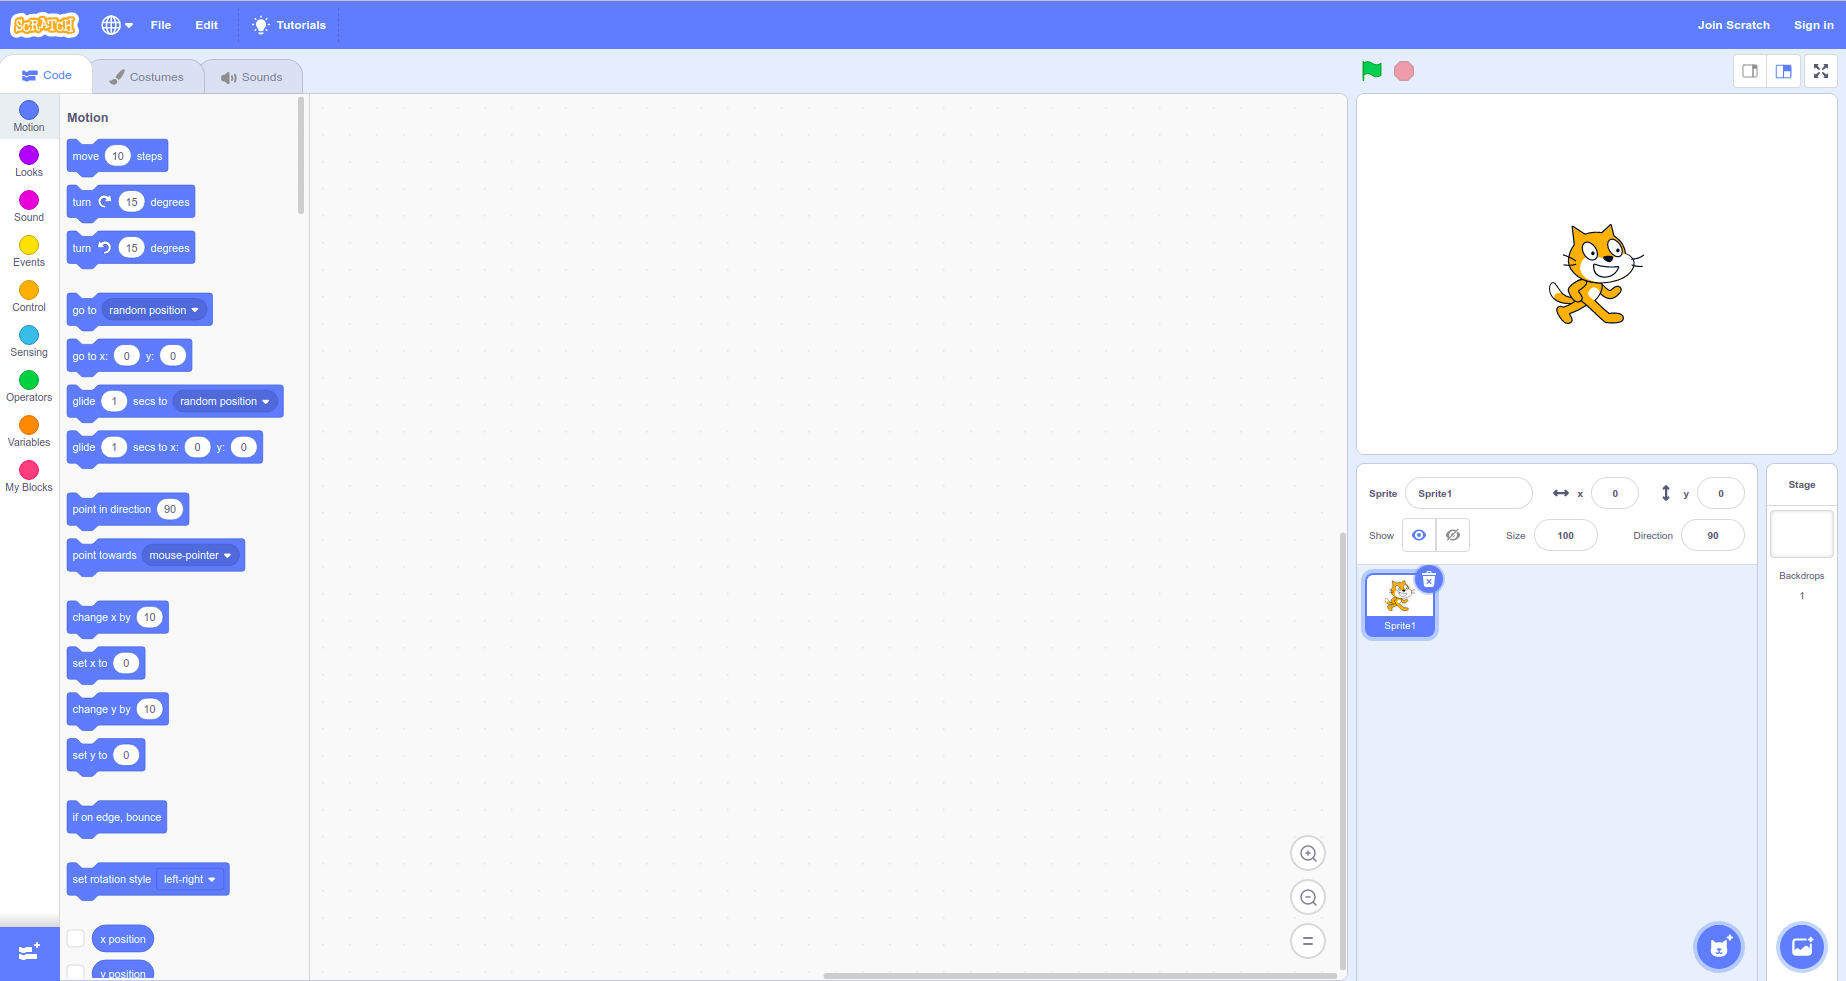
\includegraphics[width=12cm, keepaspectratio]{img/scratch.png}
    \caption{Plataforma Scratch}
    \label{fig:scrach}
\end{figure}

\begin{itemize}
\item \textbf{Snap!}\footnote{https://snap.berkeley.edu/}: Está basada en el código de programación de Scratch, creada en la Universidad de Berkeley. Esta aplicación la puedes utilizar tanto \textit{online} como descargándola y pudiendo utilizarla sin necesidad de Internet. La principal diferencia con Scratch es que te permite crear tus propios bloques utilizando JavaScript y así poder formar tu librería propia, también se puede crear listas avanzadas donde se puede almacenar cualquier tipo de dato incluso otras listas.  Esta aplicación web permite aprender a programar de una manera más visual y evitando los errores de sintaxis que se podrían cometer. Snap tiene una gran comunidad de usuarios que suben sus proyectos donde se puede aprender de ellos \cite{app}.


\begin{figure}[H]
    \centering
    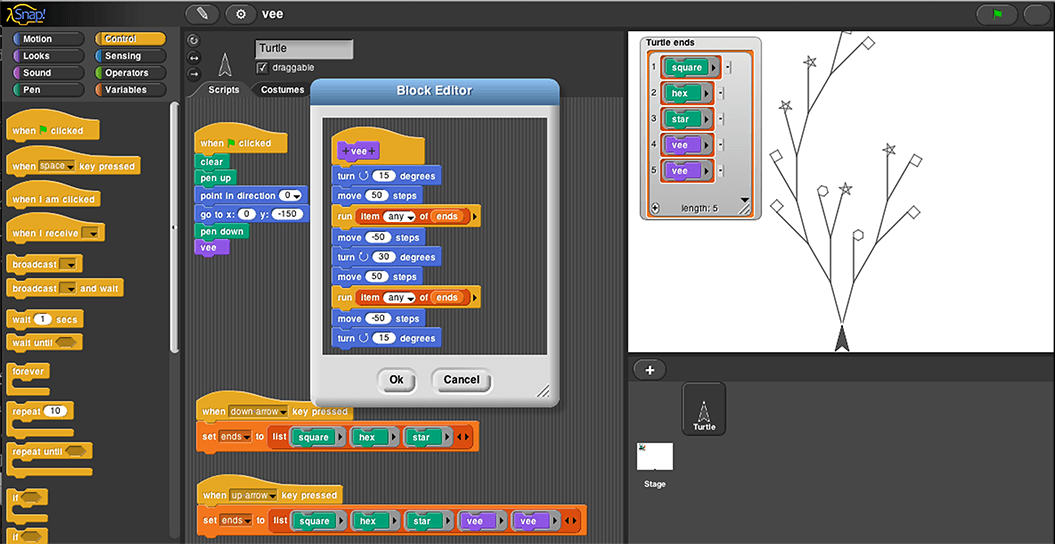
\includegraphics[width=10cm, keepaspectratio]{img/snap.png}
    \caption{Snap!}
    \label{fig:snap}
\end{figure}

\item\textbf{Robocode}\footnote{https://robocode.sourceforge.io/}: Es un videojuego multiplataforma que consiste en la creación de un tanque robot el cual tendrá que atacar y esquivar otros tanques para no ser destruido. No es necesario descargar ningún software adicional aparte del propio Robocode. Está dirigido para aprender Java y .NET. Nos podemos encontrar ligas donde las batallas de los robots transcurren en tiempo real, éstas están divididas en diferentes categorías dependiendo del tamaño de código efectivo en bytes para que sean competiciones más justas. Se puede programar las tres partes del tanque que son: el cuerpo que se encarga de mover el tanque, el radar que detecta a los adversarios y el cañón que se utiliza para apuntar y disparar. La aplicación dispone de un editor de texto, un \textit{debugger} y un compilador, todos los robots que se vayan desarrollando se podrán guardar para futuras batallas \cite{app}.


\begin{figure}[H]
    \centering
    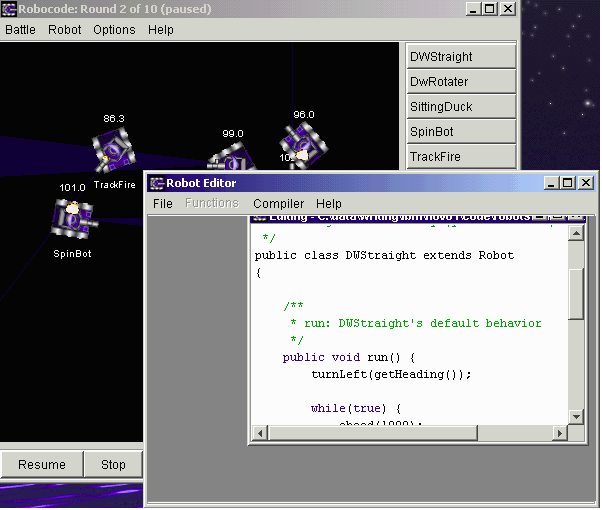
\includegraphics[width=7cm, keepaspectratio]{img/Robocode.png}
    \caption{Robocode}
    \label{fig:robocode}
\end{figure}


\item \textbf{CodeCombat}\footnote{ https://codecombat.com/}: Es una página web donde a través de un personaje se enseña a programar en diferentes lenguajes como Python, JavaScript, C++, entre otros. El objetivo del juego es ir superando los diferentes niveles, los cuales van aumentando de dificultad. Está compuesto por 110 niveles gratuitos con opción de jugar más niveles si se paga, además pagando se pueden desbloquear diferentes héroes, aprender a programar juegos y páginas web\cite{app}.
\end{itemize}

\begin{figure}[H]
    \centering
    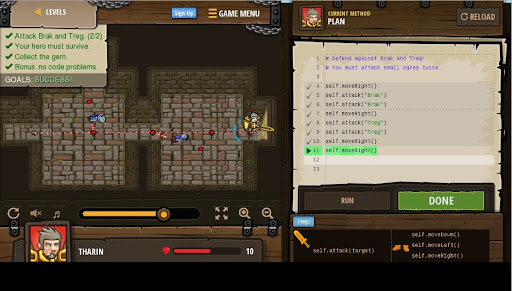
\includegraphics[width=13cm, keepaspectratio]{img/Codecombat.jpg}
    \caption{CodeCombat}
    \label{fig:codecombat}
\end{figure}

\section{Robótica y software de robot}
La robótica es la ciencia o rama tecnológica encargada del estudio, diseño, creación y aplicación de los robots. En la actualidad existen muchas formas de estudiar robótica, puedes estudiarla tanto en universidades como en cursos. Existen diferentes herramientas para poder trabajar con robots, como los sistemas operativos robóticos. Se encuentran varios ejemplos de sistemas operativos como RoboComp\footnote{https://robocomp.github.io/web/} o Player\footnote{http://playerstage.sourceforge.net/}, pero el más conocido y usado es ROS\footnote{https://www.ros.org/} (\textit{Robot Operating System}).\\

ROS es un \textit{framework} flexible para escribir \textit{software} de robots. Las principales ventajas son que es de código abierto, contando con una comunidad global para mejorar el \textit{software}. Además, es una herramienta multiplataforma e independiente de la administración del \textit{backend} y las interfaces de usuario \cite{ros}.\\

El funcionamiento de ROS está basado en nodos, éstos son procesos ejecutables que realizan una tarea simple. Las tareas de los nodos pueden ser controlar la velocidad, el motor de las ruedas o la localización. Los nodos pueden enviar mensajes o recibir mensajes de otros nodos a través de los tópicos. \\

Los tópicos se encargan de transmitir el mensaje a todos los nodos que se han suscrito y reciben los mensajes que publican los nodos. Los nodos no saben que nodo ha publicado ni que nodo se ha suscrito a un tópico. Los nodos también pueden ofrecer servicios que serán acciones que otro nodo puede pedir. El servidor que ofrece el servicio solo manda la respuesta cuando recibe una solicitud de otro nodo, haciendo la comunicación síncrona. En la Figura \ref{fig:ros} se muestra un esquema del funcionamiento de ROS \cite{ros2}.\\

Otro nodo importante es el nodo maestro que se encarga de registrar todas las suscripciones y publicaciones a los tópicos.\\

\begin{figure}[H]
    \centering
    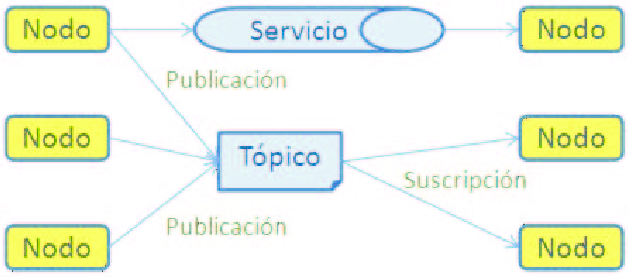
\includegraphics[width=12cm, keepaspectratio]{img/ros.png}
    \caption{Esquema ROS}
    \label{fig:ros}
\end{figure}
\newpage
Para programar robots, otra herramienta potente son los simuladores de robots. Permiten emular a robots reales de forma virtual para poder trabajar con ellos. La simulación es importante para saber cómo se comportaría un robot en la realidad y saber si necesita cambios. Además, una ventaja es que económicamente la construcción de un robot puede ser costosa, con un simulador se evitan estos gastos.\\

Existen varios simuladores como CoppeliaSim\footnote{https://www.coppeliarobotics.com/}, antiguamente llamado V-REP, cuenta con un entorno de desarrollo integrado. Cada objeto o modelo se puede controlar vía ROS, un \textit{plugin}, un \textit{script} integrado, un cliente API remoto o una solución personalizada \cite{sim}.  Webots\footnote{https://cyberbotics.com/} es otro simulador de código abierto y multiplataforma, ofrece bibliotecas con muestras de mundos, sensores o robots, entre otras características \cite{körber2021comparing}.\\

Entre todos los simuladores cabe destacar Gazebo\footnote{http://gazebosim.org/}. Para crear su simulación dinámica utiliza cuatro motores diferentes: ODE\footnote{\textit{open dynamics engine}} (simulación de cuerpos rígidos, que permite detectar y simular colisiones), Bullet (simulación de cuerpos rígidos y blandos, también detecta colisiones), DART\footnote{\textit{Dynamic Animation and Robotics Toolkit}} (simulación de la dinámica y cinemática de un robot) y Simbody (herramienta útil para simular articulaciones con restricciones y resuelve la segunda ley de Newton) \cite{upm56724}.\\

Gazebo representa gráficos 3D avanzados y realistas utilizando OGRE\footnote{\textit{Object-Oriented Graphics Rendering Engine}}, que facilita la \textit{renderización}. Dispone de diferentes sensores con la opción de añadir ruido. Además, se puede desarrollar complementos para los robots, los sensores o el ambiente. Gazebo ofrece varios robots o la posibilidad de crear uno propio \cite{gaz}.
\newpage
\section{Plataformas de programación de robótica}
Una parte de la robótica es la programación de estos robots por lo que se han ido creando herramientas de aprendizaje sencillas y atrayentes para el usuario. En Internet se pueden encontrar diversas plataformas web las cuales te enseñan sobre programación y robótica, como es el caso de Unibotics. Entre ellas se encuentran:

\begin{itemize}
\item \textbf{TheConstruct}\footnote{https://www.theconstructsim.com/}: Plataforma web que enseña sobre robótica, ROS e inteligencia artificial. Tiene una versión gratuita en la que se ofrecen tres cursos: Linux para robótica, Python3 para robótica y C++ para robótica, si se quiere puedes acceder a todos los cursos con su versión de pago. Está desarrollado para que puedan utilizarlo tanto principiantes como profesionales. No requiere de la instalación de ROS. Además, una de sus ventajas es que tiene una gran comunidad donde se puede establecer contactos y aprender nuevas formas de programar robots. TheConstruct cuenta con robots reales que se pueden alquilar por un determinado tiempo, dando la posibilidad de poder conectarse a ellos y programarlos desde cualquier lugar. Una vez se selecciona un curso, se tiene en la parte izquierda la teoría para realizar el curso. También tiene un interfaz de usuario dónde se escribe el código, un terminal para escribir comandos y una simulación del robot que se va a programar.

\begin{figure}[H]
    \centering
    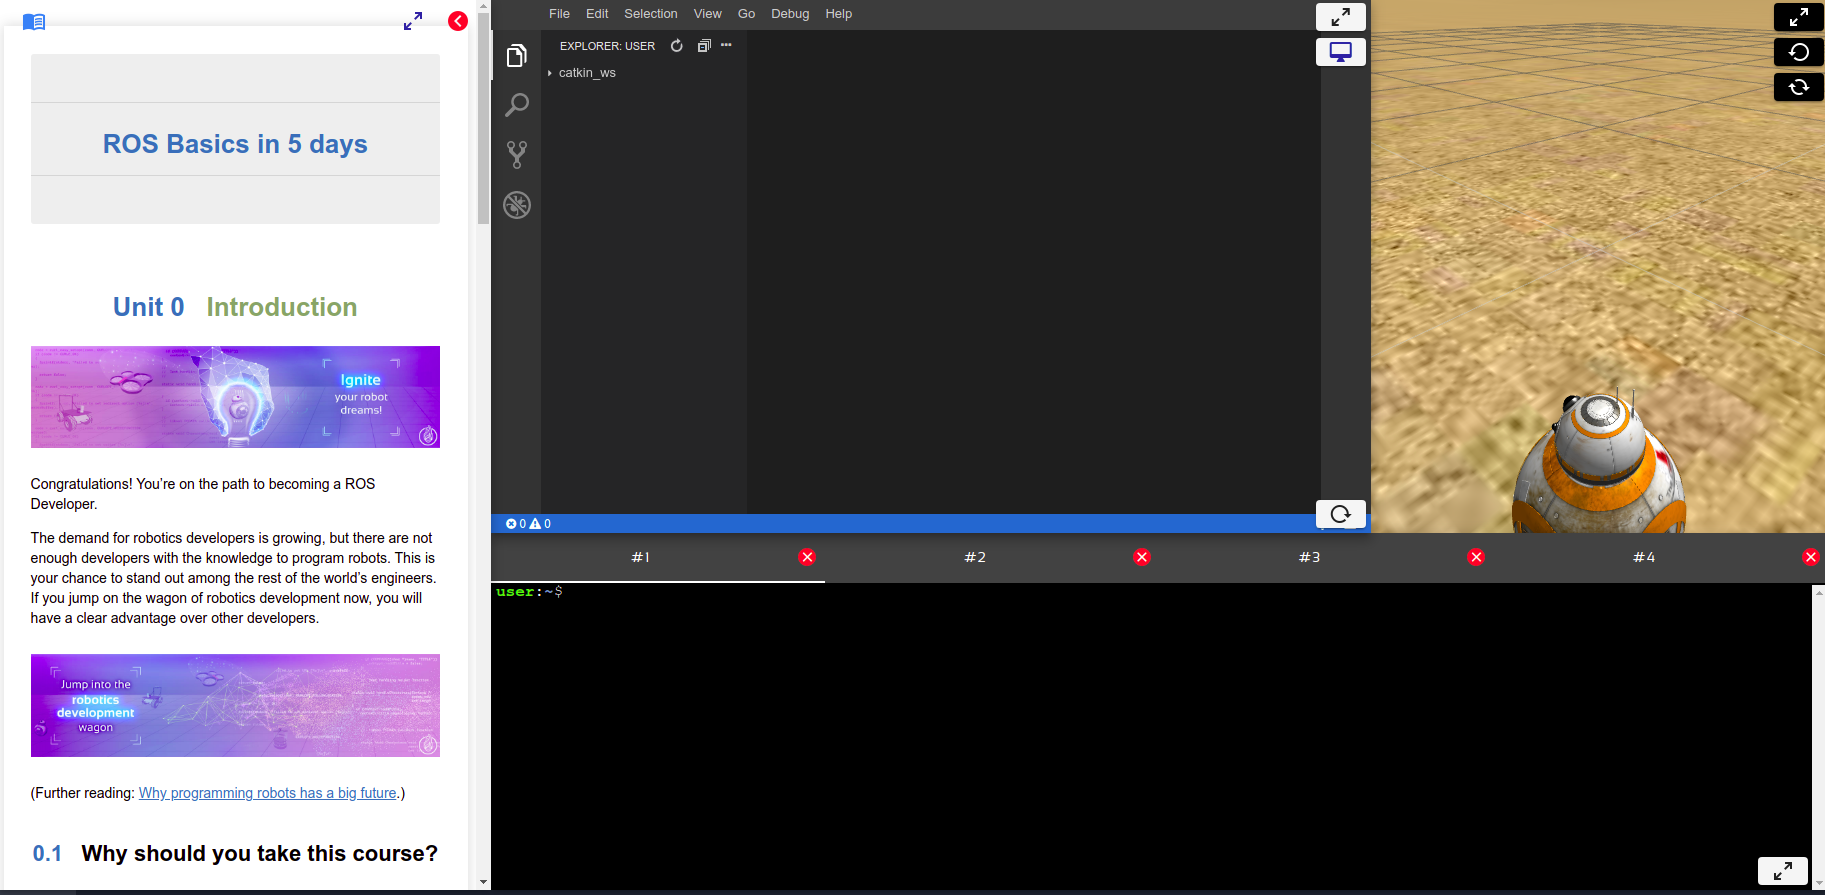
\includegraphics[width=12cm, keepaspectratio]{img/theconstruct.png}
    \caption{Curso en TheConstruct}
    \label{fig:construct}
\end{figure}
\newpage
\item \textbf{Riders.ai}\footnote{https://riders.ai/}: Plataforma robótica de simulación, educación y competencia basada en la nube, desarrollada por Acrome Robotic Systems \cite{riders}. Es una plataforma de pago, solamente es gratis la primera lección del curso Introducción a la robótica: parte 1. Consta de otros dos cursos, los cuales son la continuación del curso mencionado anteriormente. Además, una vez finalizados los cursos se obtiene un certificado. Se enseña a programar en Python o C++ los robots.  Las lecciones están formadas por la teoría, el interfaz de usuario y el simulador Gazebo, todo ello en la misma pestaña como se muestra en la figura \ref{fig:riders}.  Riders dispone de dos ligas para competir con otros programadores. Una liga consiste en drones voladores y otra sobre robots móviles.
\begin{figure}[H]
    \centering
    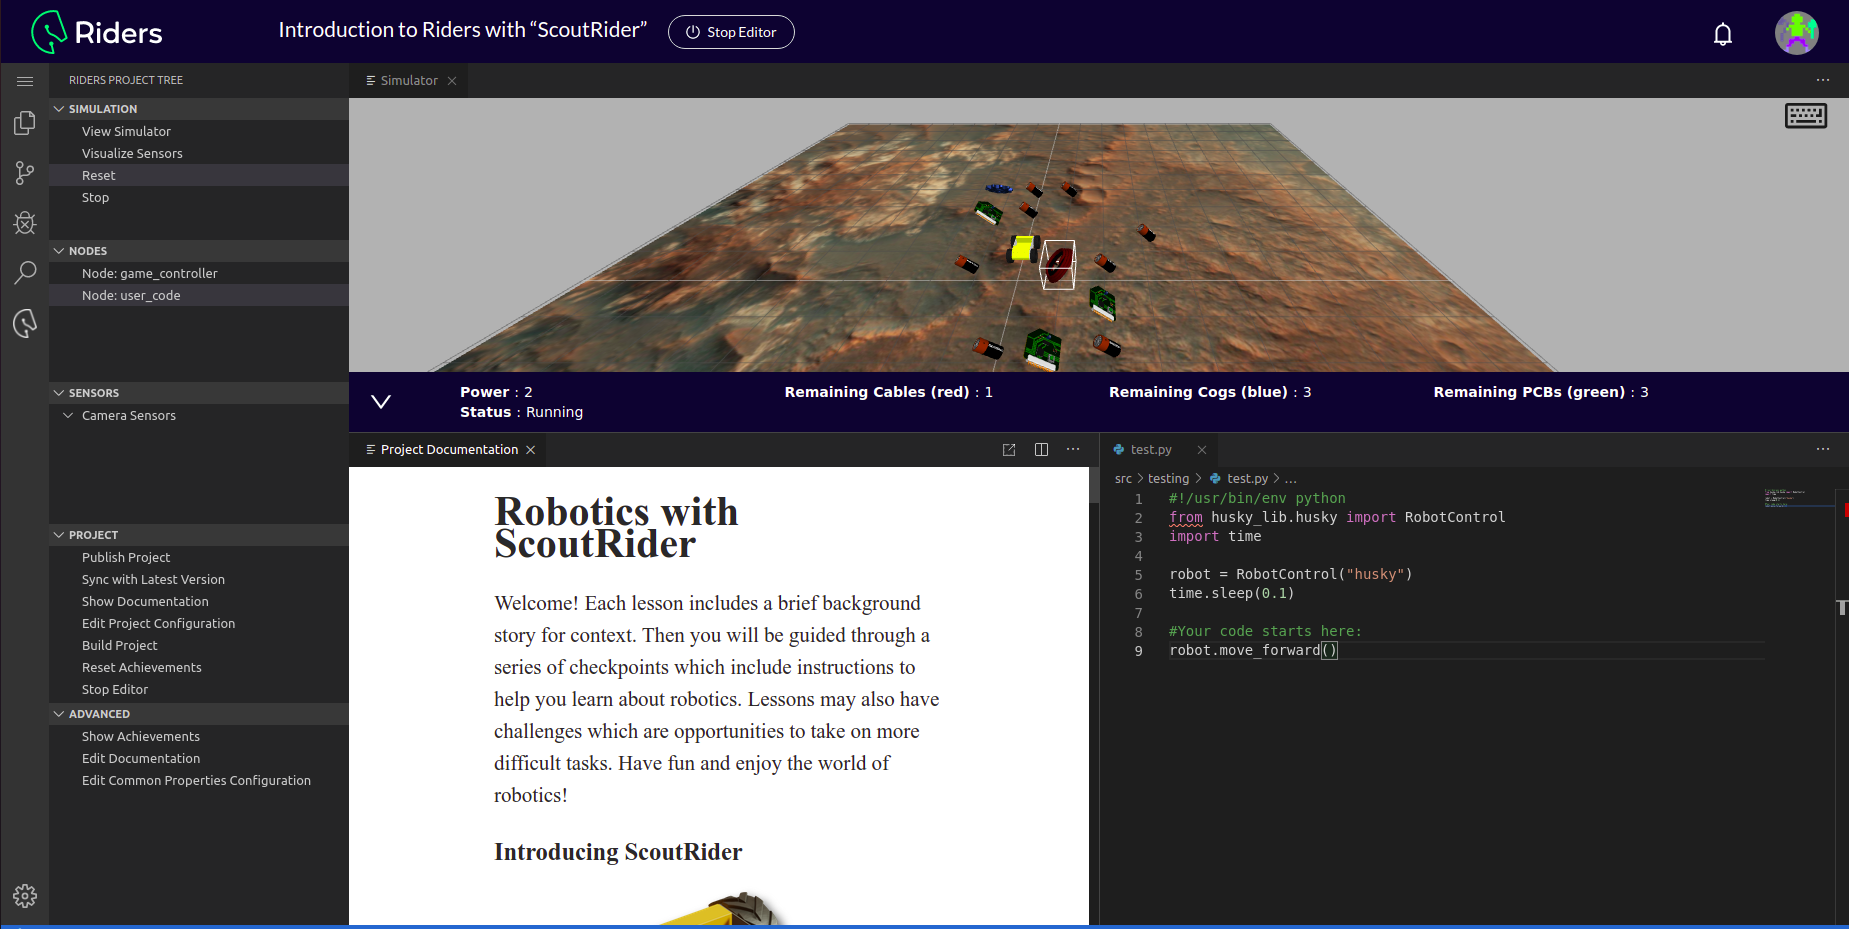
\includegraphics[width=12cm, keepaspectratio]{img/riders.png}
    \caption{Curso en Riders.ai}
    \label{fig:riders}
\end{figure}
\end{itemize}
\section{Unibotics}

Unibotics\footnote{https://unibotics.org/} es una plataforma en línea de robótica educativa donde se desarrolla este Trabajo de Fin de Grado, en la cual se enseña a programar de una manera llamativa y divertida para estudiantes universitarios. Unibotics proviene de otra plataforma que no está en línea, llamada Robotics Academy\footnote{http://jderobot.github.io/RoboticsAcademy/}. Ambas plataformas han sido creadas por la asociación de robótica e inteligencia artificial, JdeRobot.\\


La plataforma consta de varios ejercicios que se pueden dividir en ejercicios de \textbf{conducción autónoma} (\textit{Follow Line}, \textit{Obstacle avoidance}, \textit{Global Navigation}, \textit{Car Junction} y \textit{Autoparking}), \textbf{robots de servicios }(\textit{Vacuum Cleaner}, \textit{Localized Vacuum Cleaner} y \textit{Laser Mapping}), \textbf{drones} (\textit{Drone Cat and Mouse} y \textit{Rescue People}) y \textbf{visión artificial} (\textit{3D Reconstruction}, \textit{Color Filter}, \textit{OpticalFlow Teleop} y \textit{Montecarlo Visual Loc}).\\

Se puede programar los ejercicios directamente desde la web sin la necesidad de instalar software adicional. En cada ejercicio, el usuario puede introducir código fuente, cargarlo en el cerebro de un robot simulado, ejecutarlo en simulación y visualizar el interfaz gráfico. Además, se puede subir o guardar el código realizado y comprobar la eficacia y el estilo del código. Se utiliza el lenguaje Python para poder realizar los ejercicios. Unibotics utiliza una imagen de Docker llamada RADI \footnote{https://hub.docker.com/r/jderobot/robotics-academy/}(\textit{Robots Academy Docker Image} donde están preinstaladas las dependencias y así no se tiene que descargar nada localmente. Está basada en ROS y Gazebo \cite{robotics}.\\

\begin{figure}[H]
    \centering
    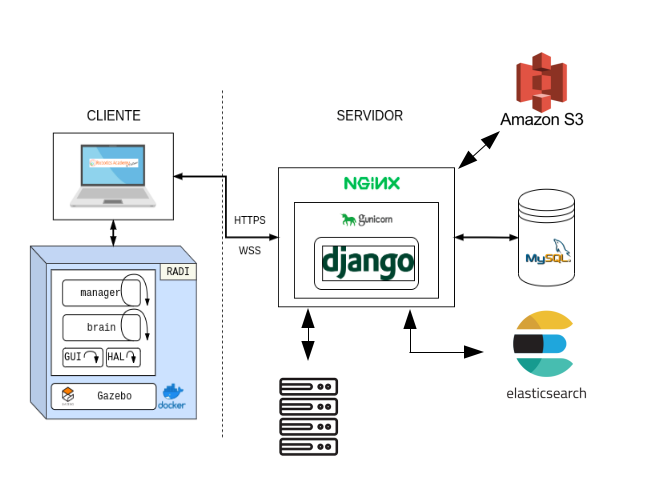
\includegraphics[width=13cm, keepaspectratio]{img/infraestructura.png}
    \caption{Infraestructura de Unibotics}
    \label{fig:infra}
\end{figure}
En la Figura \ref{fig:infra} se muestra la infraestructura de la plataforma actualmente. En la parte del servidor se encuentra un \textit{webserver}, el cual se conecta a base de datos como Elsaticsearch y MySQL, también se conecta al almacenamiento de la nube de Amazon S3 y una granja de 80 puestos. En la parte del cliente, a parte de la plataforma web se conecta a través de tres websocket al contenedor Docker, RADI. Esto hace que el coste computacional del simulador sea menor.\\

En los últimos 5 años se ha recibido ayuda de \textit{Google Summer of code}\footnote{https://summerofcode.withgoogle.com/archive/}, gracias a la cual se han ido añadiendo contenidos a la plataforma y también gracias a Trabajos de Fin de Grado.\\

En la actualidad esta plataforma es utilizada en las asignaturas de Robótica móvil y Robótica de servicios en el grado de Ingeniería de Robótica Software de la universidad Rey Juan Carlos y en el máster de visión artificial de la misma universidad.

\begin{figure}[H]
    \centering
    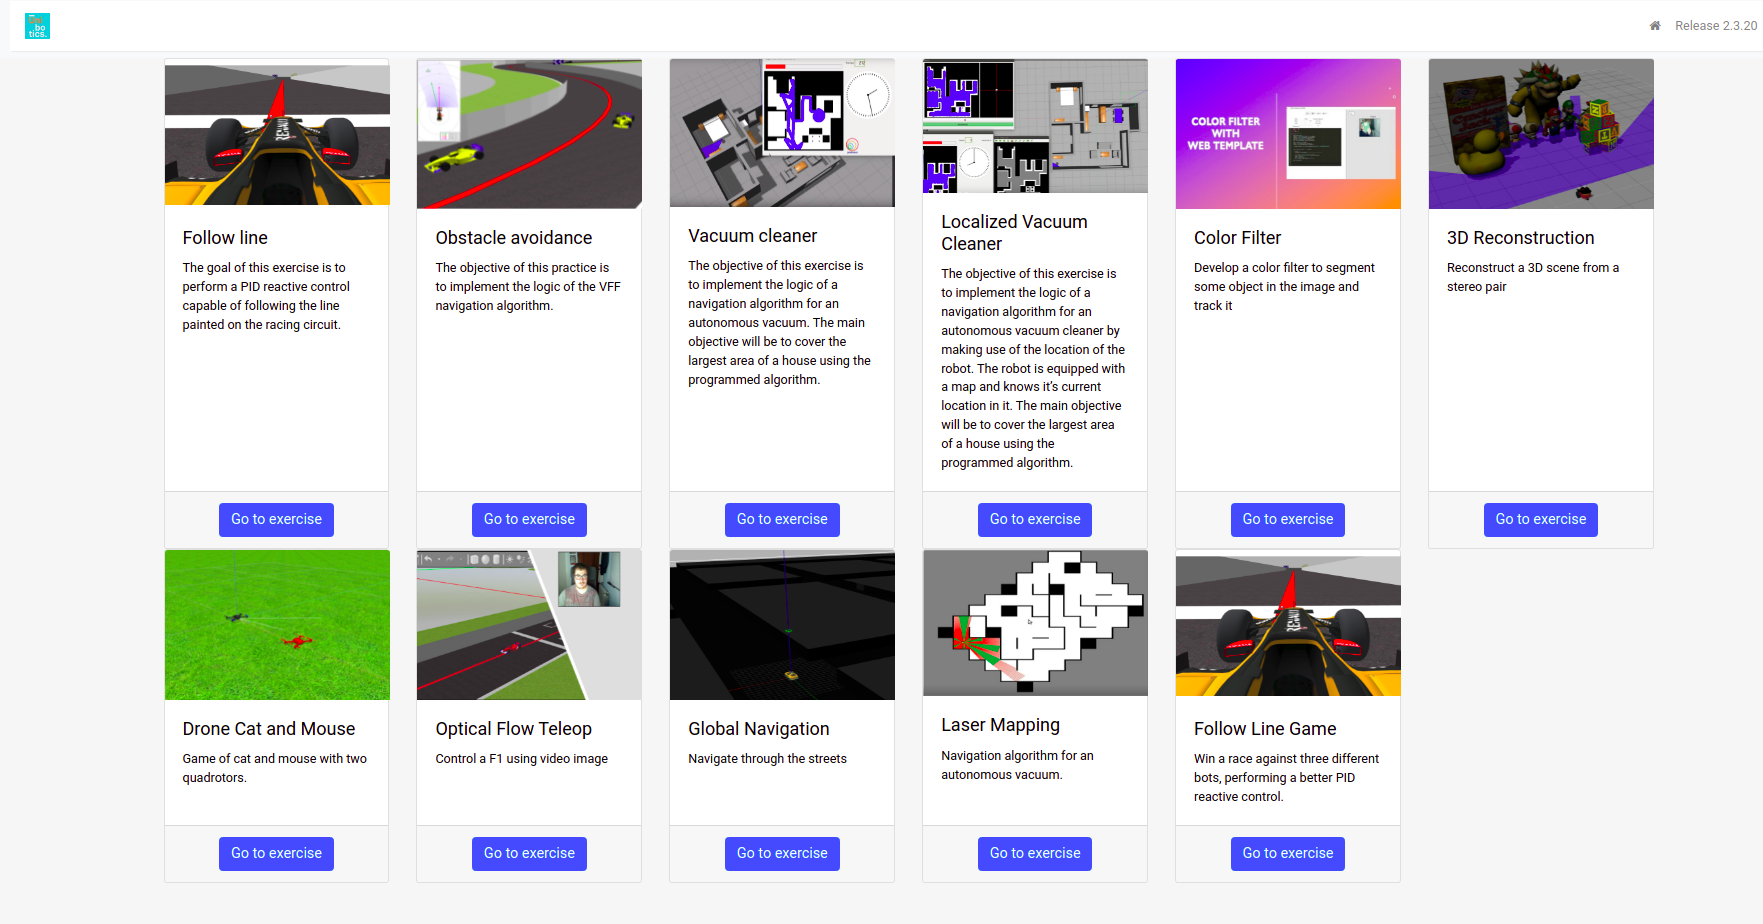
\includegraphics[width=15cm, keepaspectratio]{img/unibotics.png}
    \caption{Unibotics en la actualidad}
    \label{fig:unibotics}
\end{figure}

\section{Estructura del documento}

Este Trabajo de Fin de Grado consta de los siguientes capítulos:

\begin{itemize}
    \item \textit{Capítulo 1 Introducción}: introducción a las tecnologías web, a páginas web educativas sobre robótica y Unibotics antes de la realización de este TFG.
    \item \textit{Capítulo 2 Objetivos y Metodología}: Descripción de los diferentes objetivos a cumplir en el TFG y la metodología seguida para la realización de estos.
    \item \textit{Capítulo 3 Herramientas utilizadas}: se describen las diferentes tecnologías web utilizadas en este trabajo y las herramientas usadas para la recogida y grabación de datos y la visualización de estadísticas automáticas.
   \item \textit{Capítulo 4 Analíticas de Elasticsearch y Dash}: en este capítulo se expone el diseño y la implementación de la recogida de sondas y su posterior visualización en la plataforma de Unibotics.
  \item \textit{Capítulo 5 Conclusiones}: se desarrollan las conclusiones de los resultados obtenidos en este TFG, además de las competencias que se ha adquirido y futuros trabajos que se podrían realizar a partir de este.
   \end{itemize}